\scanpage{6}

% Main 01: reused typescript strip, running bottom to top at the left.
\[
\underline{\mathrm B}=(\text{Gr-stacks})\qquad
\widehat{\underline{\mathrm B}}\qquad
\underline{\mathrm B}(\unsure{0|\mathrm O})^{\wedge}
\]
commutes not only with arbitrary projective limits, but equally with arbitrary direct limits, or what amountsto the same, that direct limits in the category (Gr-stacks) can be computed component-wise. (Here \(\underline{\mathrm B}(0)\) stands for the full subcategory of \(\underline{\mathrm B}\) formed by the basic objects \(\underline{\mathrm D}_n\), \(n\ \underline{\mathrm N}\) .)
% The repeated typed 0 uses the first candidate of the same retained 0/O doubt.

\handwritten{
% Main 02: the isolated D is doubled; the live indexed D is plain.
\[
\widetilde{\mathbb D}\qquad
\unsure{\mathscr N|N}\longmapsto
\overset{\deleted{\unsure{I_n|D_n}}}{\widetilde D_n}
\]

% Main 06: the lower leading relation is a new main-reader doubt.
\[
\begin{aligned}
&1+n\mathbin{.}2^1+\frac{n(n-1)}{2}\,2^2\ \text{---}\ +2^n\\
&\qquad\unsure{>|=}(1+2)^n=
\end{aligned}
\]

% Main 03: three distinct rightward shafts and heads.
% Main 04: the down arrow ends over n, with membership and I in the next cell.
\diagram{\begin{tikzcd}[ampersand replacement=\&,row sep=1.15em,column sep=.35em]
\widetilde D_{n'}\arrow[r,bend left=38]\arrow[r]\arrow[r,bend right=38]
 \&[1.65em] \widetilde D_n \& {}\\
 \& \widetilde D_n\arrow[d] \& {}\\
 \& n \& {\in\begin{tikzpicture}[baseline=(downI.base),x=1em,y=1em]
\node[anchor=base,inner sep=0pt] (downI) at (0,0) {$\mathbb I$};
% Literal detached triangular point above, slightly left of the I stems.
\fill (-.065,.93)--(-.025,1.005)--(.025,.945)--cycle;
\end{tikzpicture}}
\end{tikzcd}}

% Main 05: both upper I forms are doubled; the old qualifier remains uncertain.
\[
\begin{aligned}
d_n\in\widetilde D_n&\longrightarrow\deleted{N}\mathbb I
 &\qquad d_n&\longmapsto n\\
&\text{strictement}\\
&\text{croissante}\\
&\text{image \unsure{est|\(\subset\)}}\ \mathbb I_{\deleted{\unsure{\in n|<n}}\leq n}
\end{aligned}
\]

% Main 09 and 10: detached traces, preserved without assigned lexical meaning.
\figure{\begin{tikzpicture}[line width=.5pt,line cap=round,line join=round]
% Main 09: slight rise at the entry of the upper short trace.
\draw (0,0)..controls(.025,.025)and(.06,.02)..(.13,.015);
% Main 10: point above-left, uneven rule, weak interval, angular terminal return.
\fill (2.61,-1.15) circle[radius=.018];
\draw (2.68,-1.23)..controls(2.78,-1.21)and(2.89,-1.25)..(2.94,-1.25);
\draw[line width=.18pt] (2.94,-1.25)--(2.975,-1.25);
\draw (2.985,-1.25)--(3.005,-1.28)--(3.03,-1.25);
\end{tikzpicture}}

% Main 07: margin note written sideways; both membership arches open downward.
% First live eta/g/y and xi/f/x doubts govern the later repeated candidates.
% Local limits remain eta/y over the middle J, xi/x over the last J,
% and xi/x/f at the lower endpoint; the repeated xi and eta do not resolve them.
\margin{\resizebox{.99\marginparwidth}{!}{\begin{minipage}{17em}
\diagram{\begin{tikzcd}[ampersand replacement=\&,column sep=1.3em,row sep=.65em]
J_{n''}\arrow[r,"{\unsure{u_\eta|u_g|u_y}}"] \&
 {\overset{\substack{\eta\\\rotatebox{-90}{\(\in\)}}}{J}_{n'}}
 \arrow[r,"{\overset{\deleted{\unsure{u_\eta|u_g}}}{\unsure{u_\xi|u_f|u_x}}}"{inner sep=0pt,yshift=-.15em}]
 \arrow[dr,bend right=16,"{\unsure{u}}"{description,sloped,inner sep=0pt,fill=none}] \&
 {\overset{\substack{\xi\\\rotatebox{-90}{\(\in\)}}}{J}_{\deleted{\unsure{n'}}n}}\\
 \& \& \xi
\end{tikzcd}}
% Main 08: the two-bar equality has no written right member.
\(u_\xi u_\eta=\)
\end{minipage}}}
% The tentative diagonal u is centered on its bowed shaft, without a white backing.

% Main 11: this separate map precedes the x/y array in page order.
\[
\widetilde D_{n'}\longrightarrow\widetilde D_n
\]

% Main 12: one canceled left cluster, no separately surviving live connector.
% The common live D is at the intervening level between the two memberships.
\diagram{\begin{tikzcd}[ampersand replacement=\&,column sep=1.25em,row sep=.35em]
x'' \& {<} \& x'\arrow[dd,dash] \& {\in} \& {}\\
\deleted{\unsure{\downarrow|I|=}} \& \&
 |[xshift=-.35em]|{\begin{tikzpicture}[baseline=0pt]
\fill (0,0) circle[radius=.025em];
\end{tikzpicture}}
 \& \& {\overset{\deleted{D}}{\widetilde D_n}}\\
y'' \& {<} \& y'\arrow[d,dash] \& {\in} \& {}\\
{} \& \& n' \& \&
\end{tikzcd}}
\figure{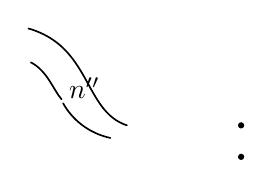
\begin{tikzpicture}[line width=.6pt,line cap=round]
% The upper arc crosses n'', which is not a free array cell.
\node[inner sep=0pt] at (.71,-.01) {$n''$};
\draw (0,.75)..controls(.8,.52)and(.7,-.3)..(1.25,-.48);
% The lower arc has a short real gap part way down.
\draw (.03,.32)..controls(.24,.21)and(.31,-.02)..(.42,-.15);
\draw (.44,-.20)..controls(.55,-.40)and(.76,-.58)..(1.04,-.64);
\fill (2.7,-.48) circle[radius=.04] (2.7,-.88) circle[radius=.04];
\end{tikzpicture}}

% Main 13: plain I, ens without a stop, and a detached point before n.
\(I\) ens ordonné

\(\mathord{\begin{tikzpicture}[baseline=-.15ex,x=1em,y=1em]
\fill (0,0) circle[radius=.03];
\end{tikzpicture}}\quad n\longmapsto\widetilde D_n\) famille d'ens ordonnés \unsure{,|;}

% Main 14: resolved old phi; a literal oblique mark above-left of the live label.
% Main 15: plain image I with a separate point below-left of its stem.
\[
\widetilde D_n\xrightarrow{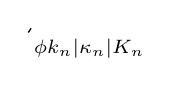
\begin{tikzpicture}[baseline=(maplabel.base),line width=.45pt]
\node[inner sep=0pt] (maplabel) {$\scriptstyle\deleted{\phi}\unsure{k_n|\kappa_n|K_n}$};
\draw ([xshift=-.18em,yshift=.22em]maplabel.north west)
 --([xshift=-.08em,yshift=.37em]maplabel.north west);
\end{tikzpicture}}I\qquad
\text{str. croiss.}\quad\text{image}\quad
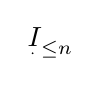
\begin{tikzpicture}[baseline=(imageI.base),x=1em,y=1em]
\node[anchor=base,inner sep=0pt] (imageI) at (0,0) {$I$};
\node[anchor=base west,inner sep=0pt] at (.2,-.3) {$\scriptstyle\leq n$};
\fill (-.08,-.24) circle[radius=.035];
\end{tikzpicture}
\]

% Main 16: the opening through K is canceled; the following capital Soit is live.
Si \(n'\leq n\), \deleted{\unsure{Soit|Sinon} l'ens \(K\)} Soit
% Main 17: left-aligned two-level definition, with a point above-left of vertical =.
\[
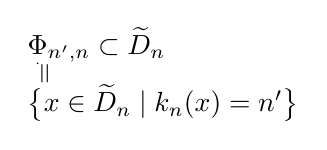
\begin{tikzpicture}[x=1em,y=1em]
\node[anchor=west,inner sep=0pt] at (0,0) {$\Phi_{n',n}\subset\widetilde D_n$};
\node[inner sep=0pt] (subseteq) at (.7,-1.05) {\rotatebox{90}{\(=\)}};
\fill (.38,-.66) circle[radius=.035];
\node[anchor=west,inner sep=0pt] at (0,-2.1)
 {$\bigl\{x\in\widetilde D_n\mid k_n(x)=n'\bigr\}$};
\end{tikzpicture}
\]
% The clean k_n carries the earlier k/kappa/K doubt; it is not a new resolution.

% Main 18: the prime and final comma both belong to the canceled phrase.
\deleted{Soit \(x\in\Phi_{n'},\)}

% Main 19: the old D group and the live B alphabet retain their ordered alternatives.
Considérons l'ens \deleted{\(\unsure{\widetilde D_{n'}|D_n}\)}\(\unsure{B|\mathbb B|\mathscr B}\)

% Main 20: plain F_0, doubled F_1 and F_2; four literal leftward arrow paths.
\diagram{\begin{tikzcd}[ampersand replacement=\&,column sep=.15em]
F_0 \& {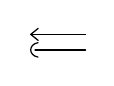
\begin{tikzpicture}[baseline=-.3ex,x=.9em,y=1em,line width=.45pt,line cap=round,line join=round]
% Upper first arrow: head joined to shaft.
\draw (2.2,.28)--(0,.28);
\draw (.3,.5)--(0,.28)--(.3,.06);
% Lower first arrow: curved left head, with a white gap before the shaft.
\draw (.29,-.02)..controls(-.1,-.08)and(-.1,-.48)..(.29,-.54);
\draw (.17,-.28)--(2.2,-.28);
\end{tikzpicture}} \& \mathbb F_1
 \& {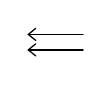
\begin{tikzpicture}[baseline=-.3ex,x=.9em,y=1em,line width=.45pt,line cap=round,line join=round]
% Both second-pair heads meet their shafts.
\draw (2.2,.28)--(0,.28);
\draw (.3,.5)--(0,.28)--(.3,.06);
\draw (2.2,-.28)--(0,-.28);
\draw (.3,-.06)--(0,-.28)--(.3,-.5);
\end{tikzpicture}} \& \mathbb F_2
\end{tikzcd}}

% Main 21: B's literal open contour, detached x, inward upper head, lower returns.
\figure{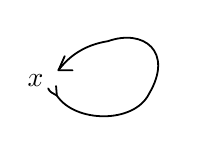
\begin{tikzpicture}[line width=.65pt,line cap=round,line join=round]
\node[inner sep=0pt] at (-.27,0) {$x$};
\draw (0,-.19)..controls(.23,-.54)and(.98,-.55)..(1.17,-.17)
 ..controls(1.49,.37)and(1.10,.66)..(.65,.50)
 ..controls(.33,.45)and(.14,.29)..(.02,.13);
\draw (.02,.13)--(.20,.13) (.02,.13)--(.10,.31);
\draw (0,-.19)--(-.01,-.07);
\draw (0,-.19)..controls(-.05,-.16)and(-.09,-.15)..(-.11,-.10);
\end{tikzpicture}}

% Main 22: headless vertical connector; a detached point below-left of the y prime.
\diagram{\begin{tikzcd}[ampersand replacement=\&,row sep=1.1em]
x'\arrow[d,dash]\\
{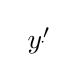
\begin{tikzpicture}[baseline=(footy.base),x=1em,y=1em]
\node[anchor=base,inner sep=0pt] (footy) at (0,0) {$y$};
\node[anchor=base,inner sep=0pt] at (.4,.35) {$\scriptstyle\prime$};
\fill (.28,.23) circle[radius=.035];
\end{tikzpicture}}
\end{tikzcd}}

% Main 23: three filled points, explicit upper arrow wings, disconnected low segment.
\figure{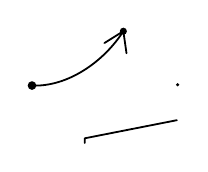
\begin{tikzpicture}[line width=.65pt,line cap=round,line join=round]
\fill (0,.15) circle[radius=.055];
\draw (0,.15)..controls(.45,.13)and(.91,.45)..(1.16,.84);
\draw (.92,.69)--(1.16,.84)--(1.20,.56);
\fill (1.16,.84) circle[radius=.045] (1.85,.16) circle[radius=.022];
\draw (.67,-.58)--(.67,-.52)--(1.84,-.29);
\end{tikzpicture}}

% Main 24: shallow broken V; the right arm itself has a second real interruption.
\figure{\begin{tikzpicture}[line width=.5pt,line cap=round]
\draw (0,.05)--(.07,0);
\draw (.11,.005)--(.145,.018);
\draw (.166,.027)--(.2,.04);
\end{tikzpicture}}

% Main 25: pi_0 and the written abbreviation/punctuation remain literal.
\[
\begin{aligned}
\pi_0(F_*,x)&=\text{ens des classes d'hom.topie. des}\\
&\phantom{=}\text{lacets en }x
\end{aligned}
\]
}% end handwriting
% archive sheet number: 5
